\section{Introduction}


\indent This technical report is intended to serve as a step by step tutorial for the replication of a prosthetic hand \cite{Kontoudis2015IROS} developed by the \href{www.openbionics.org}{OpenBionics (www.openbionics.org)} initiative \cite{Liarokapis2014ASURRW}. Based on a previous design for the OpenBionics robotic hands \cite{Zisimatos2014IROS}, the prosthetic hand was developed to be affordable, light-weight and intrinsically-compliant. The proposed design is also structurally and kinematically anthropomorphic. In particular, its sizing is parametrically determined in an anthropomorphic fashion, according to data provided by hand anthropometry studies \cite{BuchholzErgonomics1992}, allowing for personalization and adjustment to the needs of each individual. Moreover, its kinematic model is derived by incorporating an index of Anthropomorphism \cite{Liarokapis2013ICRA} in the design optimization process. Finally, the prosthetic hand bears a novel differential mechanism based on the \textit{whiffletree} or \textit{seesaw} mechanism that allows the user to switch between various postures using a single actuator. Postures and gestures selection is easy and intuitive, through the use of simple locking buttons that can independently block the motion of each finger. The proposed hands can be easily fabricated using low-cost, off-the-shelf materials and rapid prototyping techniques. 

 
In the following sections, we describe in detail all the necessary steps for the replication of the proposed prosthetic hand. In order to facilitate the fabrication for non-expert users, effort has been devoted to utilize off-the-shelf materials and equipment that can be easily found in hardware stores around the world.

\section{Prosthetic Hand Design}

In this section we present the prosthetic hand design. The hand is underactuated as all five fingers are controlled with a single actuator which is mounted on the palm. The transmission is achieved with tendons driven through low-friction tubes. A differential mechanism facilitates the execution of multiple postures and gestures with the single actuator. 

\subsection{Anthropomorphism}

Recently, Liarokapis et al. \cite{Liarokapis2013ICRA} formalized an index of anthropomorphism for quantifying the humanlikeness of robot hands in terms of motion capabilities and morphology. The index was defined as the weighted sum of workspace similarity subscores. These subscores were derived from comparisons between the robot hand and a human hand reference. Human hand anthropometry studies \cite{BuchholzErgonomics1992} were used to define the representative human hand model. The proposed index of anthropomorphism can be used in order to assess the humanlikeness of existing robot hands, or as an optimization criterion for designing a new generation of robot and prosthetic hands. We argue that anthropomorphism not only results to more aesthetically superior artifacts but also to a better performance in everyday life grasping and manipulation tasks. This conclusion was based on the simple observation that the objects surrounding us have been crafted according to the design and the capabilities of the human hand. Therefore, structurally and kinematically anthropomorphic artificial hands may be more well suited to execute a wide variety of everyday life tasks. 

Based on this observation, we used the index of Anthropomorphism to extract specifications for the design of our anthropomorphic prosthetic hand. In particular, we optimized for anthropomorphism with respect to the finger phalanges lengths and the positions/orientations of the finger base frames. The human hand reference was extracted from parametric models \cite{BuchholzErgonomics1992} that only require two human hand parameters: 1) the hand length (HL) and 2) hand breadth (HB). 

Finally, the extracted finger base frames orientations were further optimized to allow for a satisfactory Kapandji score \cite{Kapandji}. The Kapandji score is a tool that is widely used by physicians in order to evaluate a patient's thumb opposition capability by asking the subject to use their thumb to touch a set of different palm locations. Based on the locations reached, a score indicative of the thumb's opposition dexterity is determined by the Kapandji scale. This tool has lately found applications in robot hand design \cite{GrebensteinThesis}. Inspired by the aforementioned study, we used the Kapandji score as a criterion for determining the hand's kinematics in order for the thumb fingertip to be able to make contact with 1) the base frames of the remaining four fingers and 2) the tips of the index and pinky fingers. 

%\ref{baseFrames}.

%as shown in Fig. \ref{fingertips}.


\subsection{Finger Design}

Each one of the index, middle, ring and pinky fingers consists of three phalanges and three rotational Degrees of Freedom (DoF) for flexion/extension, while the thumb consists of two phalanges and two rotational DoF for flexion/extension and one rotational DoF for abduction/adduction. All joints of the fingers are flexure joints based on elastomer materials (silicone or polyurethane sheets), the sizing of which was determined empirically to achieve both a lightweight structure and a force range that is adequate for everyday life tasks \cite{DollarAR2005}. In terms of functionality, the aforementioned finger actuation and transmission is bioinspired, in the sense that it structurally replicates the flexion/extension motions of the human fingers. More specifically, the use of elastomer materials on the joints implements the passive extension, while cables (Dyneema fishing line) driven through low-friction tubes implement the flexion. Finally, in order to enhance stability through force impact absorption and increased friction at the contacts \cite{deformableciocarlie2005}, we covered the fingertips with: 1) deformable sponge-like tape , 2) rubber tape and 3) anti-slip tape.

\subsection{Palm}

The palm consists of two parallel planes that can be made out of Plexiglas (acrylic) or ABS (depending on the manufacturing technique used) and which  accommodate: 1) the finger base frames, 2) the thumb mechanism, 3) the selectively lockable differential mechanism (i.e., the whiffletree and the buttons) and 4) the actuator base. In the following sections we describe in detail the thumb locking mechanism and the selectively lockable differential mechanism.

  
\subsubsection{Thumb Locking Mechanism}

For the thumb we use a selectively lockable toothed mechanism that can implement 9 different opposition configurations as depicted in Fig. \ref{thumb}. These configurations were selected to allow the efficient execution of the Kapandji test \cite{Kapandji} and to allow also the user to switch among different grasping postures (e.g., pinch grasp, power grasp, key grasp etc.). The proposed one DoF thumb mechanism serves as a simple alternative to the mechanically complex three DoF human thumb. The proposed mechanism is completely stiff when it is locked, in contrast to the friction based mechanisms \cite{Baril} that are affected by torsional forces that are inherent in dynamic/unstructured environments (these forces can result to large, uncontrolled displacements of the thumb for these mechanisms). The thumb tendon is terminated to an appropriate servo pulley. Small motor angular displacements are required for the finger to be actuated. Finally, the diameters of the pulleys were optimized for the Kapandji test \cite{Kapandji}.

\begin{figure}[h]
%\setlength{\belowcaptionskip}{-8pt}
%\setlength{\abovecaptionskip}{-6pt}
\begin{center}
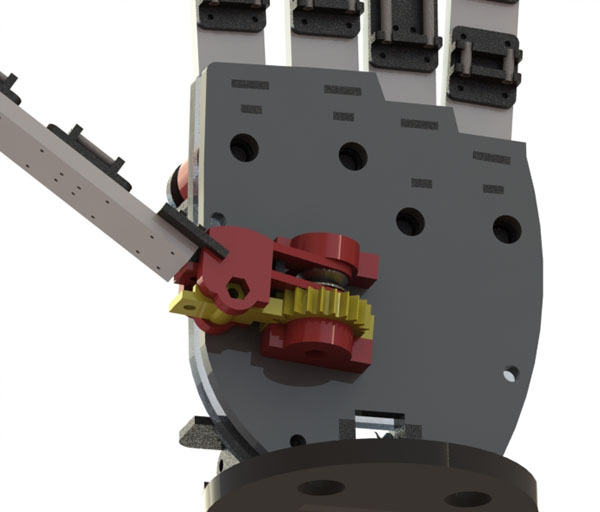
\includegraphics[width=6.4cm]{figures/paper_images/thumbmechanism.jpg}
\end{center}
\caption{The thumb mechanism consists of the red and golden parts. The red parts are mounted in appropriate slots on the robot palm to facilitate installation of the thumb mechanism. The golden parts are: 1) a pulley that routes the thumb tendon to the back of the hand and 2) the toothed, selectively lockable mechanism that allows adjustment of thumb's opposition. The robot thumb can be passively positioned by the user, in 9 discrete configurations.} 
\label{thumb}
\end{figure}

\subsubsection{A Selectively Lockable Differential Mechanism}

A selectively lockable differential mechanism connects the actuator with the tendons of each finger. The mechanism is a variation of the whiffletree \cite{Birglen}. The whiffletree consists of three bars: one bar connecting the index and middle fingers (bar 1), one bar connecting the ring and pinky fingers (bar 2) and the main bar that connects bar 1 and bar 2, as depicted in Fig. \ref{differential}. The top two bars of the whiffletree bear 2 slots each, which allow for selective independent locking of all fingers upon pressing of corresponding buttons that are mounted on the top of the palm. Intuitively, when each button is pressed, the corresponding bar slot is filled and the corresponding finger's motion is blocked. Therefore, switching among different hand postures is easy. A total of $2^4=16$ different finger combinations can be implemented and when they are combined with the 9 discrete positions of the thumb, they result to 144 distinct postures that can be achieved with a single actuator. The differential mechanism is depicted in Fig. \ref{differential} and the locking buttons in Figs. \ref{palm} and \ref{RobotHandViews}.

\begin{figure}[h]
\begin{center}
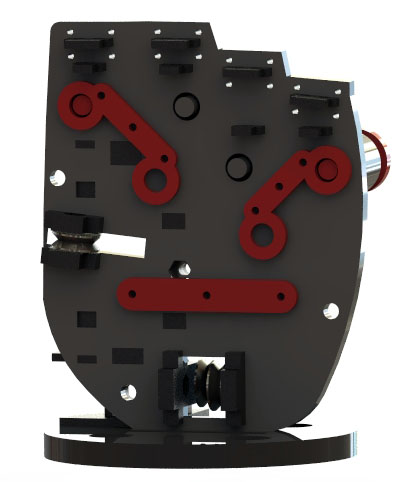
\includegraphics[width=8cm]{figures/paper_images/whiffletree.jpg}
\end{center}
\caption{Inner side of the palm. The three bars of the proposed whiffletree are depicted with red color. The holes of the upper two bars are filled by the elongated parts of the corresponding buttons, constraining the motion of different fingers. In this instance the motion of the index and pinky fingers is constrained, resulting to a change at the inclination of the differential mechanism finger bars.} 
\label{differential}
\end{figure}

\subsection{Fabrication Techniques and Personalized Design}

All files (CAD files, codes) required for the replication and control of the proposed robot hands, are available for download through the OpenBionics initiative \cite{Liarokapis2014ASURRW} website at the following URL:
\begin{center}{\small{\url{http://www.openbionics.org}}}\end{center} 

 The proposed design is essentially 2D and can be replicated with various fabrication techniques. In particular, we provide 3D models (.stl files) that can be used for fabrication with rapid prototyping techniques such as 3D printing and 2D models (.dwg, .dxf and other CAD files) that can be used for fabrication with laser cutting machines or other standard machining tools. The proposed hands are made out of off-the-shelf, low-cost materials. All required materials can be easily found in hardware stores around the world. 

 \begin{figure}[h]
\begin{center}
\begin{tabular}[50]{ c c }
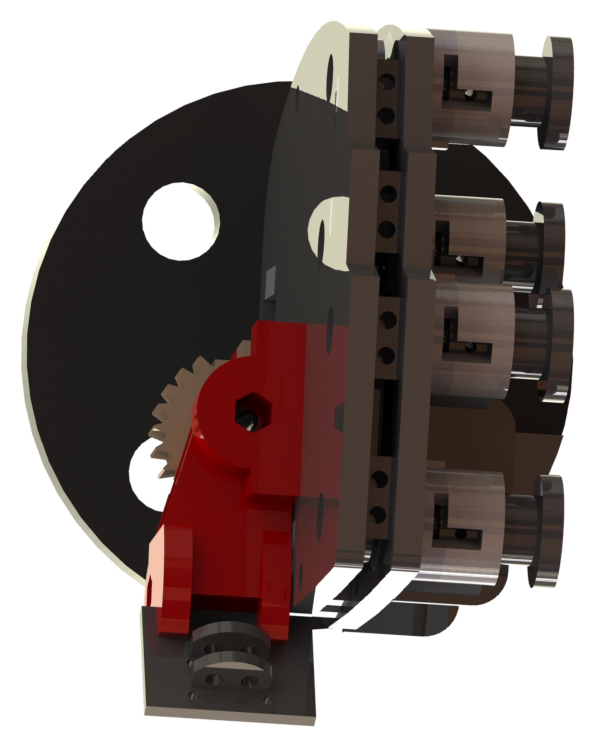
\includegraphics[height=9cm]{figures/paper_images/buttons.JPG}&
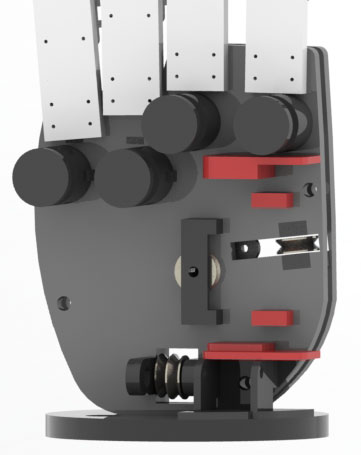
\includegraphics[height=9cm]{figures/paper_images/servobase.jpg}\\
{{a) thumb mechanism}} & {{b) servo base}}\\
\end{tabular}
\end{center}
\caption{Subfigure a) depicts the thumb mechanism in red and golden colors. Subfigure b) depicts the servo base of the HerkuleX servo motor in red. In both subfigures the buttons that implement the differential tree locking are denoted with black color.} 
\label{palm}
\end{figure} 

For reference, we provide the finger design parameters for a prosthetic hand with length 19 cm in Table \ref{fingerparameters}, while other complementary features are reported in Table \ref{handcharacteristics}. It should be pointed out that both the weight and the cost of the proposed hand design are significantly low, 300 g and $<$200 USD respectively. 

\begin{table}[ht!]
\caption{Finger characteristics for a robot hand with length 19cm} \label{fingerparameters}
\begin{center}
\begin{tabular}[50]{ c c c c c }
{\it{Finger}} & {\it{Weight}} & {\it{Length}} & {\it{Breadth}} & {\it{Width}}\\
\hline
{Index} & {30 g} & {88 mm} & {16.2 mm} & {15 mm}\\
{Middle} & {30 g} & {98 mm} & {16.2 mm} & {15 mm}\\
{Ring} & {30 g} & {95 mm} & {16.2 mm} & {15 mm}\\
{Pinky} & {25 g} & {76 mm} & {16.2 mm} & {15 mm}\\
{Thumb} & {20 g} & {68 mm} & {16.2 mm} & {15 mm}\\
\end{tabular}
\end{center}
\end{table} 

\begin{table}[ht!]
\caption{Hand characteristics} \label{handcharacteristics}
\begin{center}
\begin{tabular}[50]{ c c c c c }
{\it{Cost}} &  {\it{Weight}} & {\it{Length}} & {\it{Breadth}} & {\it{Width}}\\
$<$ 200 USD & 300 g & 190 mm & 90 mm & 62.50 mm 
\end{tabular}
\end{center}
\end{table} 

 \begin{figure}[ht]
\centering
\begin{tabular}[50]{ c c c c }
{\it{Front}} & {\it{Side 1}} & {\it{Side 2}} & {\it{Back}}\\
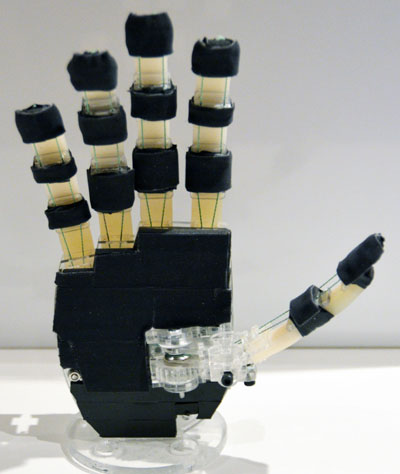
\includegraphics[height=3.4cm]{figures/paper_images/hand1.jpg}&
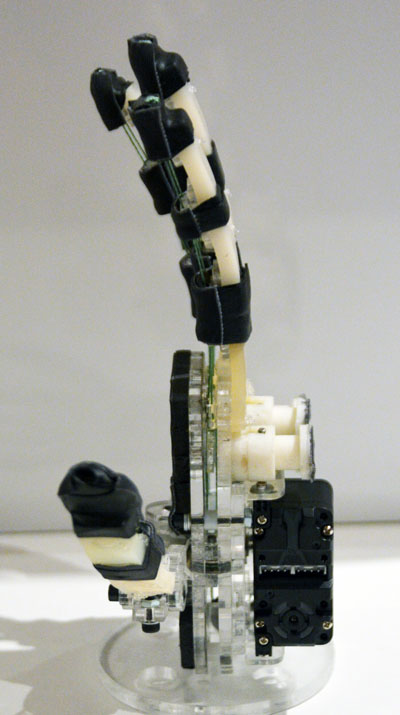
\includegraphics[height=3.4cm]{figures/paper_images/hand2.jpg}&
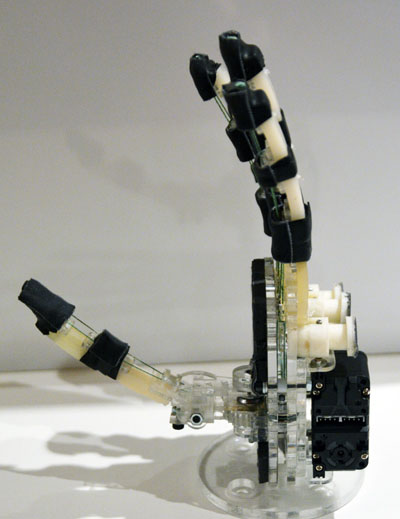
\includegraphics[height=3.4cm]{figures/paper_images/hand3.jpg}&
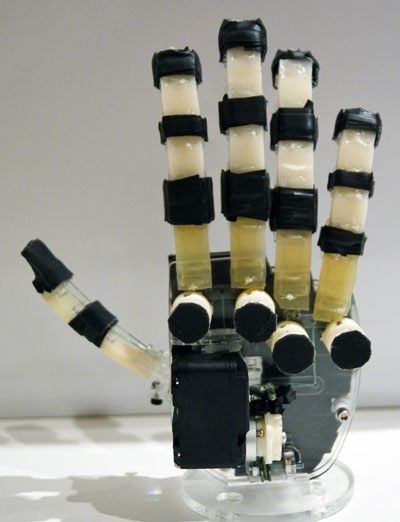
\includegraphics[height=3.4cm]{figures/paper_images/hand4.jpg}\\
\end{tabular}
\caption{Different views of the prosthetic hand developed.} 
\label{RobotHandViews}
\end{figure} 

\section{Results \& Experiments}

The performance capabilities of the proposed design have already been validated with extensive experimental paradigms that include: 1) grasping of a wide range of everyday life objects, 2) execution of a series of daily living tasks. For the experiments, we used an Arduino Micro platform \cite{Arduino} to control the HerkuleX DRS0201 servo motor, a custom made PCB module that connects the arduino platform with the servo motor and the ROS package (written in Python) that we created within the context of the OpenBionics initiative (available at \url{https://github.com/OpenBionics}). In the following sections we evaluate the performance of the proposed prosthetic hands.

\subsection{Force Exertion Capability}

Fig. \ref{forcedisplacement} contains diagrams demonstrating the relationships between the linear displacement of the tendon and the force applied at the fingertips, with and without finger blocking, for various hand postures. This can be useful for performing precision grasps, since blocking a subset of fingers leads to increased force transmission for the remaining free fingers.


\begin{figure}[h]
\centering
\begin{tabular}{ c c c }
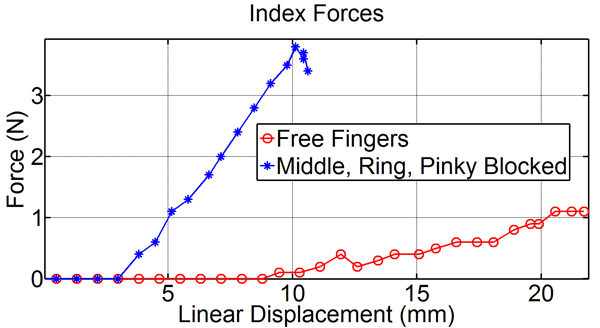
\includegraphics[scale=0.22]{figures/paper_images/indexforces.jpg} &
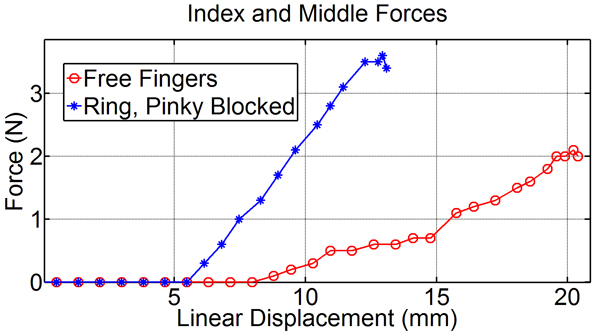
\includegraphics[scale=0.22]{figures/paper_images/indexmiddleforces.jpg} &
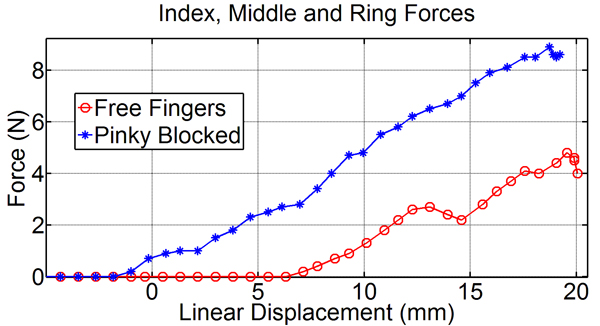
\includegraphics[scale=0.22]{figures/paper_images/indexmiddleringforces.jpg}\\ 
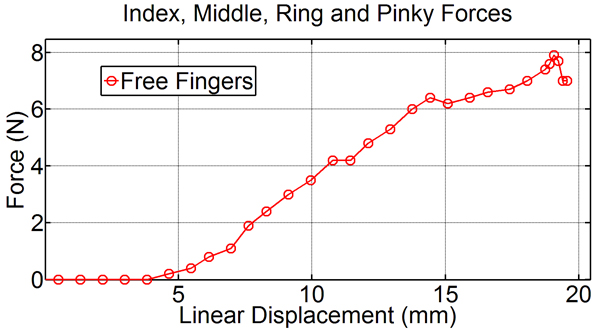
\includegraphics[scale=0.22]{figures/paper_images/fingersforces.jpg} & 
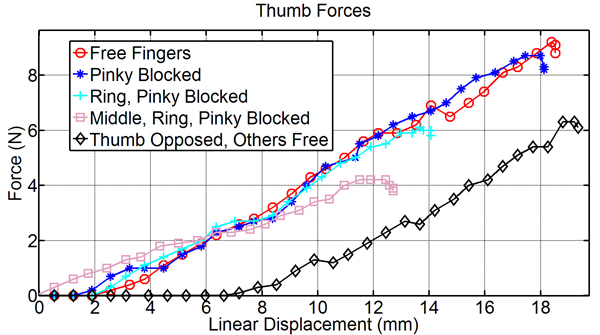
\includegraphics[scale=0.22]{figures/paper_images/thumbforces.jpg}
\end{tabular}
\caption{Relationship between tendon displacement and finger forces for various postures.} 
\label{forcedisplacement}
\end{figure}

\subsection{Implementing Various Grasping Postures and Common Gestures}

The efficacy of the selectively lockable differential mechanism was validated through a plethora of experiments.  The user was pressing the locking buttons to achieve different postures. This functionality is not only important for grasping (where the user is able to choose a preferred grasping strategy / posture), but also for: 1) implementing specific gestures (e.g., making the peace sign or showing a number), 2) reaching for an object located at a narrow space (task that might require less than five fingers), or 3) execute non-prehensile manipulation tasks (e.g., press a button or move a slider on a console). Figs. \ref{Locked} and \ref{Free} depict various postures, achieved by pressing different sets of buttons. 

\begin{figure}[ht]
\begin{center}
\scalebox{0.95}{
\begin{tabular}[50]{ c c c c }
{\it{Index}} & {\it{Middle}} & {\it{Ring}} & {\it{Pinky}}\\
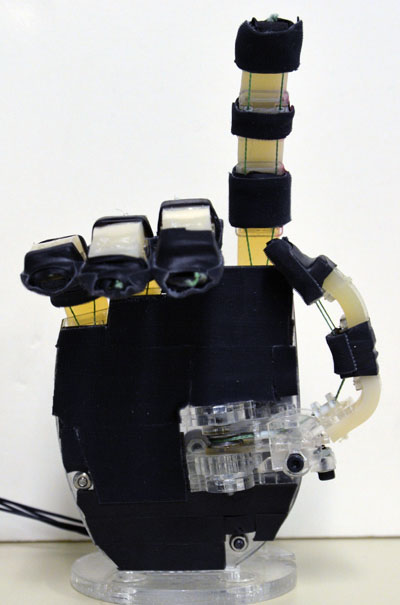
\includegraphics[height=5cm]{figures/paper_images/index.jpg}&
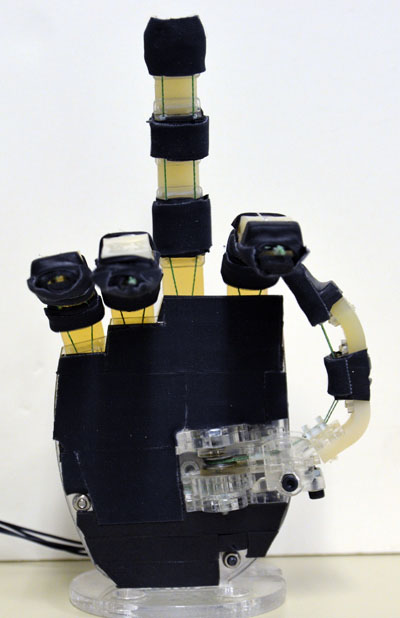
\includegraphics[height=5cm]{figures/paper_images/middle.jpg}& 
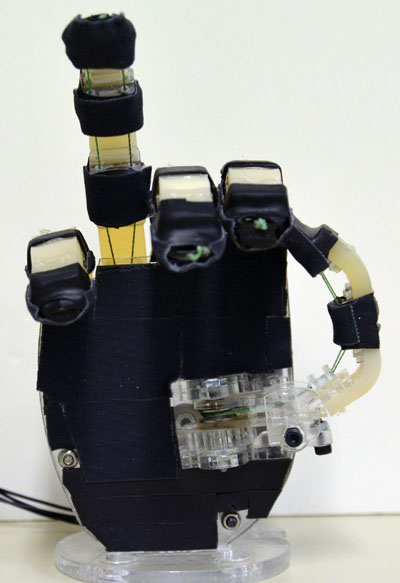
\includegraphics[height=5cm]{figures/paper_images/ring.jpg}&
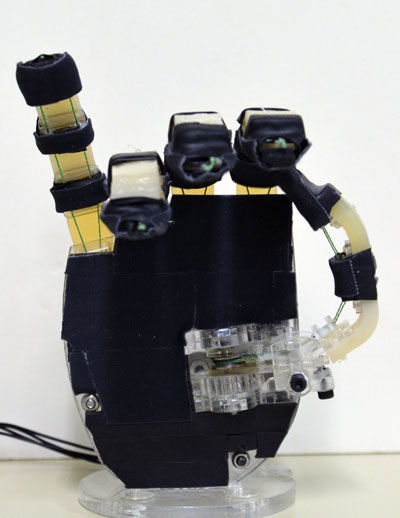
\includegraphics[height=5cm]{figures/paper_images/pinky.jpg}\\
\end{tabular}
}
\end{center}
\caption{Four different postures are depicted. All fingers except one are closing. The locked finger can be used to: 1) press buttons, 2) to reach something in narrow spaces, 3) to implement specific gestures or 4) to execute non-prehensile manipulation tasks (e.g., moving a slider).} 
\label{Locked}
\end{figure} 


\begin{figure}[ht]
\begin{center}
\begin{tabular}{ c c c c }
{\it{M, R, P}} & {\it{I, M}} & {\it{I, M, P}} & {\it{I, P}}\\
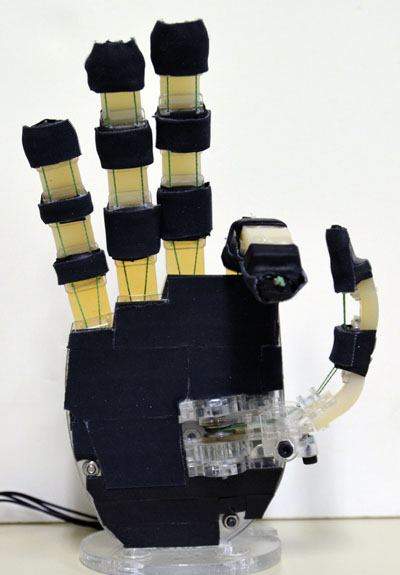
\includegraphics[height=5cm]{figures/paper_images/index_free.jpg}&
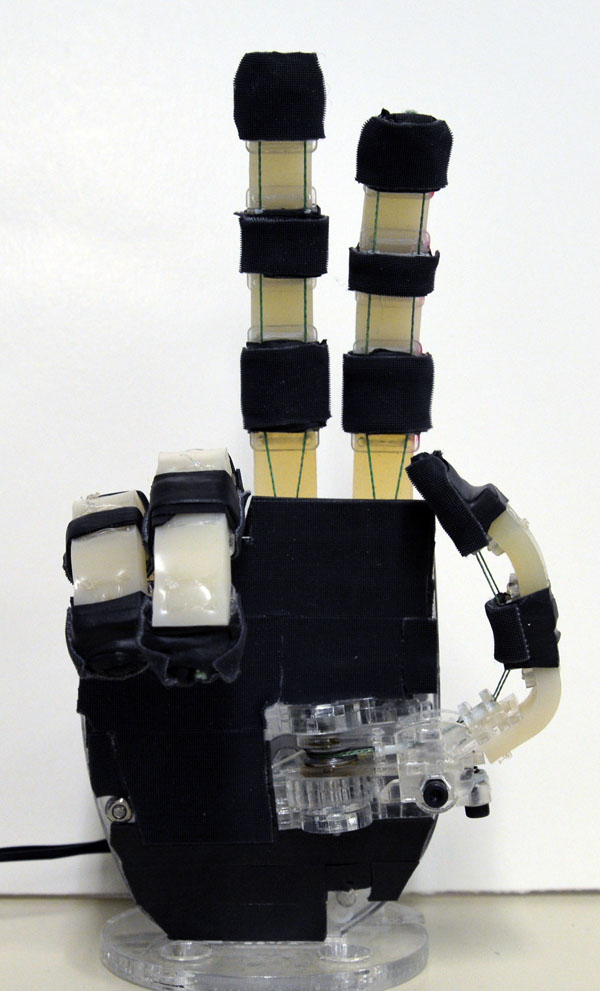
\includegraphics[height=5cm]{figures/paper_images/peace.jpg}& 
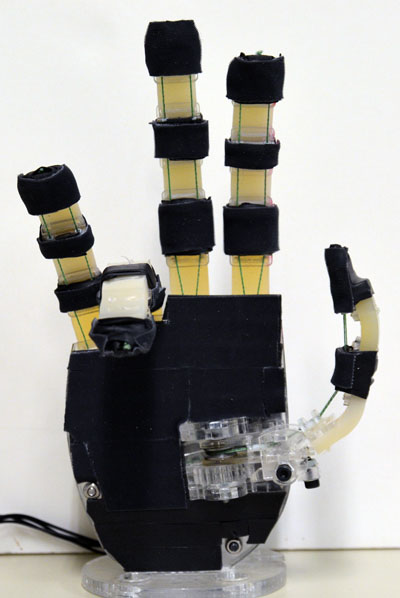
\includegraphics[height=5cm]{figures/paper_images/ring_free.jpg}&
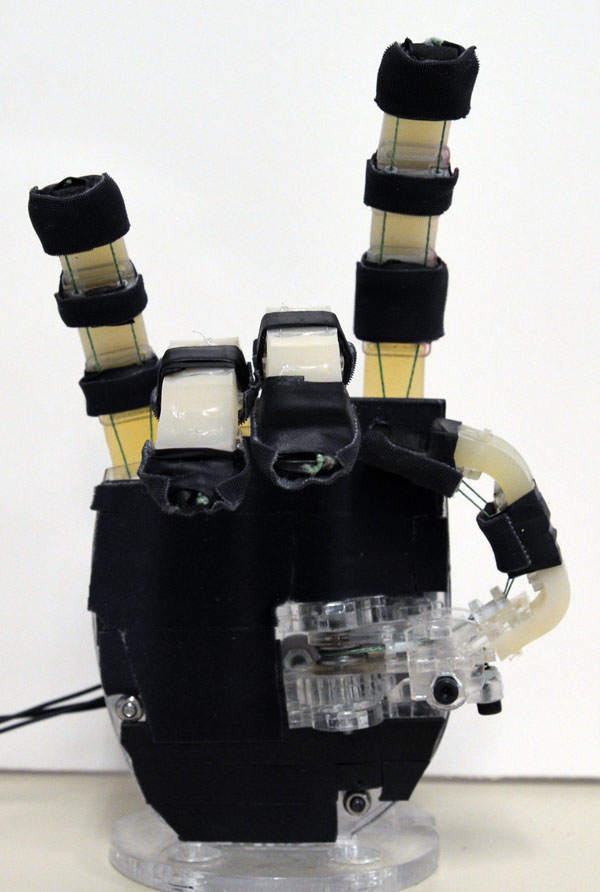
\includegraphics[height=5cm]{figures/paper_images/metal.jpg}\\
\end{tabular}
\end{center}
\caption{Four different postures are depicted. The differential mechanism allows for different grasping postures and hand gestures to be achieved. With the letters I, M, R and P we denote that motion of the index, middle, ring and pinky finger respectively, is constrained.} 
\label{Free}
\end{figure}

\subsection{Grasping Everyday Life Objects}

The actual grasping capabilities of the hand were tested through a set of experiments during which the user grasped a wide range of everyday life objects, to execute common daily living activities. For these experiments we used 1) a mug, 2) a soap, 3) a magazine, 4)  a marker, 5) a pair of glasses, 6) a large rectangular box, 7) a glass cleaner spray, 8) a 1.5L bottle of water, 9) a glass of water and 10) a spoon. Regarding the daily living tasks, the hand is used: 1) to serve water from a 1.5L bottle to a glass, 2) to stir the water inside the glass with a spoon and 3) to position a series of tools to their cases and put them inside a rectangular box. Instances of the conducted experiments are displayed in Fig. \ref{Experiments}. All experiments were recorded and the video can be found (in HD quality), at the following URL: 
\begin{center}{\small{\url{http://www.openbionics.org/videos/}}}\end{center}

More details about the experiments and the possible applications, can be found in \cite{Kontoudis2015IROS}, as well as at the official website of the OpenBionics initiative:

\begin{center}
{\url{http://www.openbionics.org}}
\end{center} 

\begin{figure}[ht!]
\centering
\scalebox{0.98}{
\begin{tabular}[50]{ c c c c }
{\it{Mug}} & {\it{Marker}} & {\it{Sunglasses}} & {\it{Bottle}}\\
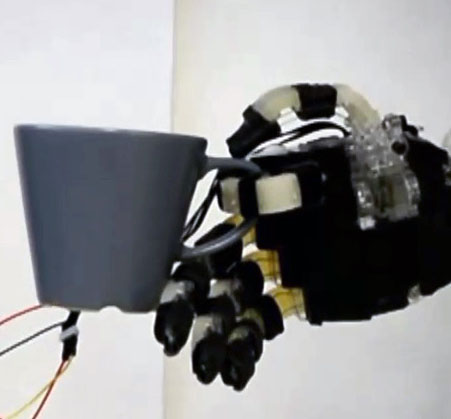
\includegraphics[height=4cm]{figures/paper_images/experiment1.jpg}&
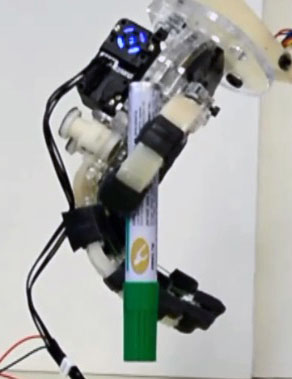
\includegraphics[height=4cm]{figures/paper_images/experiment2.jpg}&
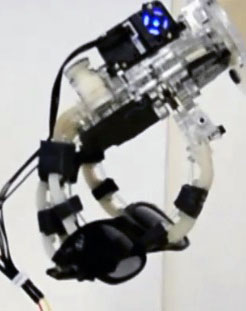
\includegraphics[height=4cm]{figures/paper_images/experiment3.jpg}&
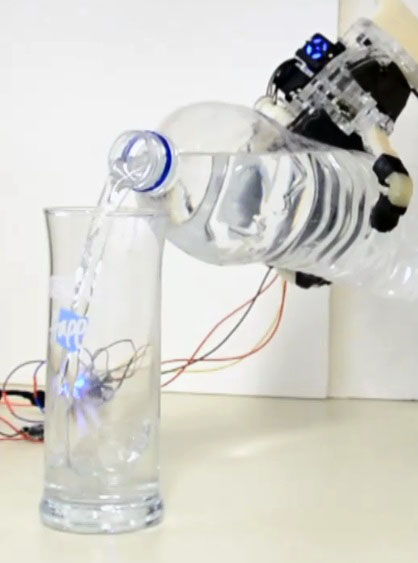
\includegraphics[height=4cm]{figures/paper_images/experiment4.jpg}\\
\end{tabular}
}
\caption{Images from the experiments conducted. Five different everyday life objects are grasped in order to execute different tasks: 1) a coffee mug is grasped from the handle in order to drink from it, 2) a marker is grasped in order to write, 3) a pair of glasses are picked up and 4) a 1.5L bottle is grasped in order to serve water.} 
\label{Experiments}
\end{figure} 

\newpage
